\documentclass[8pt]{report}
\usepackage{fullpage}
\usepackage{graphicx}

\usepackage[margin=0.5in]{geometry}
\begin{document}
\textbf{Authors}: Patrick O'Connell (oconne16) \& Jahnvi Patel (jpate201)
\begin{enumerate}
\item What is your data and task (including data preprocessing steps)? \\
Dataset for this project is acquired from \textit{Young People Survey} from \textit{kaggle.com}. The main task of the project is to predict a person's "Empathy" as either "very empathetic" or "not very empathetic". The dataset provided in the .csv files is either numerical or categorical. The numerical values were sorted based on 0 being the least and 5 being the most. While, the categorical data was sorted more delicately based on specific keywords (i.e. "never smoked" = 0, or "doctorate degree" = 5). The empty fields were filled with the total average of the column. After loading and cleaning up the data, we normalized the data so all the caregories can have the same scale for a fair comparison between them. 

\item What ML solution did you choose and, most importantly, why was this an appropriate choice?\\
 We used variety of algorithms to see which algorithm would run best with the given dataset. Ultimately, Random Forest gave us the best results with a testing accuracy of 79\%, approximately 15\% better than the baseline. 

\item How did you choose to evaluate success, including baselines, experimental setup (e.g., \% train/dev/test), metrics?\\
Experimental Setup: Train, validation and test dataset were chosen based on rule-of-thumb discussed in class. Given 1010 responses, 810 were chosen as training data, 100 were chosen as validation data and the remaining 100 responses were set aside as test data. 
Success of the algorithm is based on its performance compared to the baseline collected. If the algorithm performs better than the baseline accuracy then it is marked as a success. 

\item What software did you use and why did you choose it?

\item What are the results?
\begin{figure}[h]
  \centering
  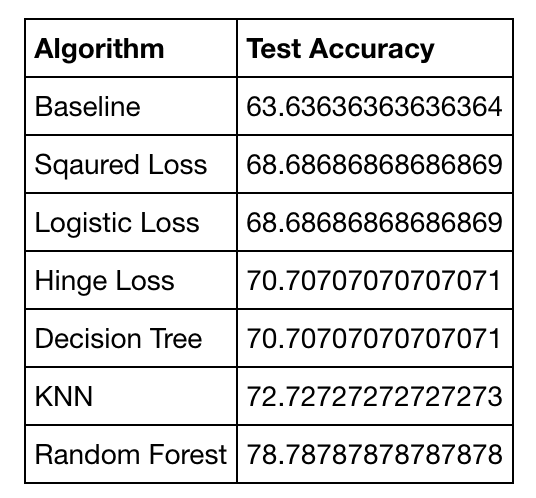
\includegraphics[height=2in]{results.png}
  \caption{Testing Accuracy of "empathetic" vs "not very empathetic"}
  \label{f:myplotfig}
\end{figure}

\item Show some examples from the development data that your approach got correct and some it got wrong: if you were to try to fix the ones it got wrong, what would you do?

\end{enumerate}
\end{document}